\documentclass[10pt]{beamer}

\usetheme[progressbar=frametitle]{metropolis}
\usepackage{appendixnumberbeamer}
\usepackage{amsmath}

\usepackage{booktabs}
\usepackage[scale=2]{ccicons}

\usepackage{pgfplots}
\usepgfplotslibrary{dateplot}

\usepackage{xspace}
\newcommand{\themename}{\textbf{\textsc{metropolis}}\xspace}

\title{67301 - MULTI ROBOT SYSTEMS - Spring 2021}
\subtitle{Final project presentation}
\date{}
\author{Tamer Ghattas}
\institute{
The Hebrew University of Jerusalem School of Computer Science and Engineering
}
% \titlegraphic{\hfill\includegraphics[height=1.5cm]{logo.pdf}}

\begin{document}

\maketitle


\section{Single-agent dirt collection}

\begin{frame}{Single-agent dirt collection}
\begin{itemize}
    \item {\bf Problem description:} collect as many as possible dirt pieces from an unknown environment without having the option of sensing the dirt. 
    \item That can be translated to: we need to cover diverse areas in the room in the shortest period of time.
    \item The problem is hard because with the time limitation we often inherit an upper bound for the area coverage.
    \item An exhaustive approach to the solution would be moving sequentially along every accessible point known from the map in hand completing a perfect coverage.
\end{itemize}
\end{frame}


\begin{frame}{Single-agent dirt collection}

We model the problem as a graph $G=(V, E)$ where the nodes $V$ represent a pixel in the map and $E$ an edge existing between every adjacent pair of pixels (nodes).


\bigskip


Our suggested solution takes the graph as input and derive goals for the robot aiming for diverse area coverage.
\end{frame}


\begin{frame}{Single-agent dirt collection}

We implemented our approach using image processing manipulations on the given map:
\graphicspath{{images/}}
\begin{itemize}
    \item First we generate binary image from the map structure.
    \item Then we perform Euclidean Distance Transform on the image.
    \item Now, we have range of gray levels that are distributed among pixels as a function of their distance of the nearest black pixel, i.e the nearest wall.
    \bigskip
    
    \begin{figure}[htp]
    \centering
    \includegraphics[height=3cm,width=4cm]{map}
    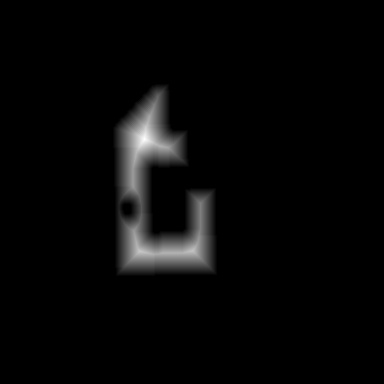
\includegraphics[height=3cm,width=4cm]{edt_img}

    \label{fig:galaxy}
\end{figure}
    
\end{itemize}
\end{frame}


\begin{frame}{Single-agent dirt collection}

\graphicspath{{images/}}
\begin{itemize}
    \item By quantizing the EDT image according to grey levels into a selected number of partitions, we get a complete partition of the room.
    \item Then, we sample from each part, a number of points which are set as goals the robot travel to using move-base node.
    \item Note that by increasing the resolution of the sampling we can guarantee more area coverage.
    \item In the following images, we can see the different parts and the sampled goals it yields (in orange): 
    
    \bigskip
    \begin{figure}[htp]
    % \centering
    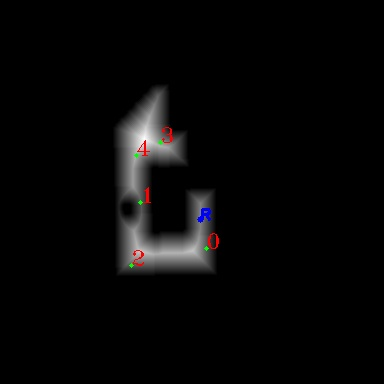
\includegraphics[height=3cm,width=3cm]{edt_img_circs_1}
    \includegraphics[height=3cm,width=3cm]{edt_img_circs_2}
    \includegraphics[height=3cm,width=3cm]{edt_img_circs_3}
    \includegraphics[height=3cm,width=3cm]{edt_img_circs_4}

    \label{fig:galaxy}
\end{figure}
    
\end{itemize}

\end{frame}


\begin{frame}{Single-agent dirt collection}

\begin{itemize}
    \item This approach was the second, first I thought about using Zig-Zag pattern with a randomly sampled angle on each turn but that is prone to missing parts of certain room structures.
    \item The presented approach on average, covers all parts of the room after enough time.
    \item A good approach might be to partition the map into compact clusters and run Zig-Zag like pattern on each.
\end{itemize}

\end{frame}


\section{Single-agent inspection}
\begin{frame}{Single-agent inspection}
\begin{itemize}
    \item {\bf Problem description:} explore a room and count the number of statically positioned spheres subject to a time limit. 
    \item That can be translated to: cover all the accessible areas using the agent sensors range and register the spheres positions within the given time frame.
    \item The problem is hard because, first, exploring is a hard problem and second, detecting sphere using a low quality 2d bird view of the sensors reading is challenging.
    \item An exhaustive approach to the solution would be using BFS/DFS algorithm to map the room including the existing static objects like the spheres.
\end{itemize}
\end{frame}

\begin{frame}{Single-agent inspection}
    We model the problem as a walk-by-wall using PD controller to keep a distance from the wall and gradually increase this reserved distance after each full circle and registering the spheres positioned along the way.
    
    PD formulation:

\begin{align*} 
&\omega(t)=K_{P} e(t)+K_{P} \frac{d e}{d t}\ \ \ \ s.t\\
&\omega(t)\text{ - PD output }\\
&K_{P}\text{ - proportional gain }\\
&de\text{ - change in error value }\\
&dt\text{ - change in time } 
\end{align*}    

\end{frame}


\begin{frame}{Single-agent inspection}
We implemented our approach using PD output for movement and the local cost map  for spheres count. For every relevant sensor reading:
\graphicspath{{images/}}
\begin{itemize}
    \item Adjust linear velocity according to distance from front wall.
    \item Adjust angular velocity according PD output.
    \item Process local cost map image and detect circles using Hough transform.
    \item For each detected circle center, register centers in a set to prevent counting twice.
    \bigskip
    
    \begin{figure}[htp]
    % \centering
    \includegraphics[height=3cm,width=3cm]{gazibo.JPG}
    \includegraphics[height=3cm,width=3cm]{sphere_img_0 (4).jpg}
    \includegraphics[height=3cm,width=3cm]{sphere_img_1 (2).jpg}

    \label{fig:galaxy}
\end{figure}
\end{itemize}
\end{frame}

\begin{frame}{Single-agent inspection}
\begin{itemize}
    \item I thought about generating a global map using local cost map registration but that isn't needed for the mere task of counting the spheres.
    \item The presented approach, did manage to fulfill the task of counting spheres with a miss count of up to 1.
    \item An improvement to the solution is to break dependency from the wall kept distance.
\end{itemize}
\end{frame}

\section{Multi-agent dirt collection}
\begin{frame}{Multi-agent dirt collection}
\begin{itemize}
    \item {\bf Problem description:} compete against another agent in collect as many as possible dirt pieces positioned in known locations to both agents, with the option of listening to to rival plans. 
    \item That can be translated to: an agent needs to maximize a utility function of the collected dirt pieces number in the existing competitive setting.
    \item Although one agent can listen to the next step of the other, the problem is challenging because the rival's whole strategy is unknown. Therefore, to gain advantage, the agent strategy has to assume rival level of strength and rationality.
    \item A safe assumption might be that the rival is rational, and will go in the near optimal path to collect the dirt pieces.
\end{itemize}
\end{frame}


\begin{frame}{Multi-agent dirt collection}

We model the problem as two decision Trees, one for each agent, $T_{Agent_{i}} = (V_{Agent_{i}},E_{Agent_{i}})$ where:
\begin{itemize}
\item Every node is a goal, a physical location of a dirt piece.
\item Each parent node in the tree has all the remaining dirt pieces (goals) as children.
\item A leaf represents collecting all the published dirt pieces.
\item Each edge $E_{Agent_{i}}=(v_{1},v_{2})$ cost is the Move-Base path length between $v_{1}$ and $v_{2}$.
\item The utility of an agent is defined for path $p\in E^{\# dirts}$ as
\item $$u(p) = \sum_{e \in p} cost(e) $$
\item A path $p^{*}$ is optimal if $$u(p^{*}) = max_{\forall p}{u(p)} $$
\end{itemize}
\end{frame}


\begin{frame}{Multi-agent dirt collection}
\graphicspath{{images/}}
We implemented the approach by:
\begin{itemize}
\item Sorting the dirt pieces locations by the length of the Move-Base planned path to goal.
\item Listen to the rival goal planing.
\item Move to the goals according to the sorted sequence.
\item If the agent heading to an impossible to arrive-before-rival goal, skip and go for the next in line.
\bigskip
\begin{figure}[htp]
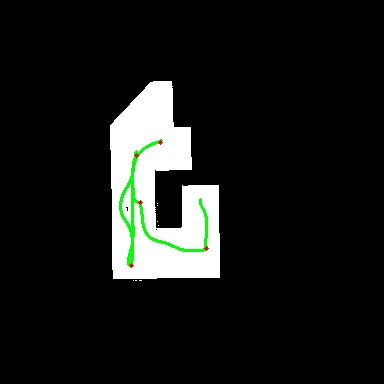
\includegraphics[height=4cm,width=4cm]{agent_0_route_img.jpg}
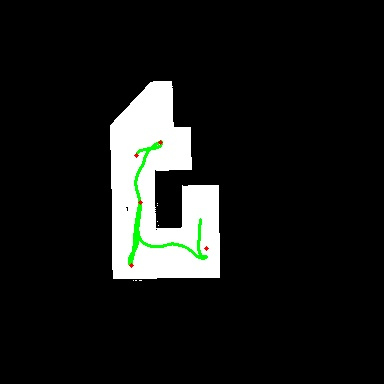
\includegraphics[height=4cm,width=4cm]{agent_1_route_img.jpg}
\label{fig:galaxy}
\end{figure}
\end{itemize}
\end{frame}

\begin{frame}{Multi-agent dirt collection}

\bigskip
In some runs, a more naive approach as simply sorting dirt pieces according to euclidean distance from initial location and going sequentially, won the more sophisticated agent. 
That is probably due to the added overhead of computing the goal as it involves the planner which might be slow.
\end{frame}

\section{Multi-agent inspection}
\begin{frame}{Multi-agent inspection}
\begin{itemize}
    \item {\bf Problem description:} explore a room and count the number of statically positioned spheres using two agents subject to a time limit. 
    \item That can be translated to: cover all the accessible areas using the agent sensors range and register the spheres positions within the given time frame.
    \item The problem is hard because, like with the single agent,  exploring is a hard problem and detecting sphere using a low quality 2d bird view of the sensors reading is challenging but what complicates it even more is managing the two agents.
    \item An exhaustive approach to the solution would be using both agents to perform BFS/DFS algorithm to map the room including the existing static objects like the spheres and cross validate correctness.
\end{itemize}
\end{frame}

\begin{frame}{Multi-agent inspection}
    Same as with single agent: We model the problem as a walk-by-wall using PD controller to keep a distance from the wall and gradually increase this reserved distance after each full circle and registering the spheres positioned along the way.
    
    PD formulation:

\begin{align*} 
&\omega(t)=K_{P} e(t)+K_{P} \frac{d e}{d t}\ \ \ \ s.t\\
&\omega(t)\text{ - PD output }\\
&K_{P}\text{ - proportional gain }\\
&de\text{ - change in error value }\\
&dt\text{ - change in time } 
\end{align*}    

\end{frame}

\begin{frame}{Multi-agent inspection}
We implemented our approach duplicating the logic from single agent i.e using PD output for movement and the local cost map  for spheres count. However, we make the agents go in opposite directions by rotating one of them before movement and rely on the kept distance from the other wall (left vs right), this ensures concurrent exploring by reducing the overlap.
\end{frame}

\begin{frame}{Multi-agent inspection}
For every relevant sensor reading in each agent:
\graphicspath{{images/}}
\begin{itemize}
    \item Adjust linear velocity according to distance from front wall.
    \item Adjust angular velocity according PD output.
    \item Process local cost map image and detect circles using Hough transform.
    \item For each detected circle center, register centers in a set to prevent counting twice.
    \bigskip
    
    \begin{figure}[htp]
    % \centering
    \includegraphics[height=3cm,width=3cm]{gazibo.JPG}
    \includegraphics[height=3cm,width=3cm]{sphere_img_0 (4).jpg}
    \includegraphics[height=3cm,width=3cm]{sphere_img_1 (2).jpg}

    \label{fig:galaxy}
\end{figure}
\end{itemize}
\end{frame}

\section{Conclusion}

\begin{frame}{Conclusion}
\begin{itemize}
    \item Simplicity might come as handy when designing autonomous agents. As having fast reactive controller (e.g. PID) are critical in some tasks.
    \item When designing solutions in robotics, generalizing solutions is not trivial. It is very task and environment dependant.
    \item Scaling up solutions to distributed agents might add to the problem if they have limited communications.
    \item Robots are fun.

\end{itemize}
\end{frame}

\end{document}
